%
%  overView
%
%  Created by Steven James Dean Martell on 2011-11-12.
%  Copyright (c) 2011 UBC Fisheries Centre. All rights reserved.
%
\documentclass[sans]{beamer}
%\usetheme{Madrid} % My favorite!
%\usetheme{PaloAlto}
\usetheme{Goettingen}
%\usetheme{Hannover}
%\usetheme{Boadilla} % Pretty neat, soft color.
%\usetheme{default}
%\usetheme{Warsaw}
%\usetheme{Bergen} % This template has nagivation on the left
%\usetheme{Frankfurt} % Similar to the default 
%with an extra region at the top.
%\usecolortheme{seahorse} % Simple and clean template
%\usecolortheme{beaver}
%\usetheme{Darmstadt} % not so good
% Uncomment the following line if you want %
% page numbers and using Warsaw theme%
% \setbeamertemplate{footline}[page number]
%\setbeamercovered{transparent}
\setbeamercovered{invisible}
% To remove the navigation symbols from 
% the bottom of slides%
\setbeamertemplate{navigation symbols}{} 
%
\usepackage{color}
\usepackage{graphicx}
\usepackage{listings}
%\usepackage{bm}         % For typesetting bold math (not \mathbold)
%\logo{\includegraphics[height=0.6cm]{yourlogo.eps}}
%

%Custom Color theme
\definecolor{bottomcolour}{rgb}{0.32,0.3,0.38}
\definecolor{middlecolour}{rgb}{0.08,0.08,0.16}
\setbeamerfont{title}{size=\Huge}
\setbeamercolor{structure}{fg=white}
\setbeamertemplate{frametitle}[default][center]

\setbeamercolor{normal text}{bg=black, fg=white}
\setbeamertemplate{background canvas}[vertical shading]
[bottom=bottomcolour, middle=middlecolour, top=black]

\setbeamertemplate{itemize item}{\lower3pt\hbox{\Large\textbullet}}
\setbeamerfont{frametitle}{size=\huge}
%end of color theme

%code block
\newtheorem{code}{Code}

%Table of contents at begining of each section
\AtBeginSection[]
{
   \begin{frame}
       \frametitle{Outline}
       \tableofcontents[currentsection]
   \end{frame}
}


%iscam logo
\newcommand{\iscam}{
	\raisebox{0.75ex}{$i$}%
	\textcolor{red}{\raisebox{0.25ex}{S}}%
	\textcolor{green}{\raisebox{0.00ex}{C}}%
	\textcolor{blue}{\raisebox{-.25ex}{A}}%
	\raisebox{-.50ex}{M}%
	}
%{$^i$}\textcolor{red}{S}\textcolor{green}{\small{}C}{\textcolor{blue}{\footnotesize{}A}}\textcolor{black}{$_\textnormal{M}$}}%{\raisebox{-0.7ex}{M}}%


\title[\iscam]{An Introduction to \iscam}
\author{Steven Martell}
\institute[UBC Fisheries Centre]
{
University of British Columbia \\
\medskip
{\emph{s.martell@fisheries.ubc.ca}}
}
\date{\today}
% \today will show current date. 
% Alternatively, you can specify a date.
%
\begin{document}

%
\begin{frame}
\titlepage
\end{frame}
%


%!TEX root = /Users/stevenmartell/Documents/CURRENT PROJECTS/iSCAM-trunk/docs/iSCAM-guide/overView.tex
\section{Installation} % (fold)
\label{sec:installation}


\subsection[Source code]{Obtaining source code} % (fold)
\label{sub:obtaining_source_code}

\begin{frame}[containsverbatim]
	\frametitle{Obtaining \iscam\ source code}
	Source code available at:\\
	\url{http://code.google.com/p/iscam-project/}
	\vfill
	Use subversion to checkout a copy
	\vfill
	\underline{On Mac \& Linux, in Terminal:}
	\tiny
	\begin{verbatim}
		svn checkout http://iscam-project.googlecode.com/svn/trunk/			iscam-project-read-only
	\end{verbatim}
	\normalsize
	\vfill
	\underline{On Windows use a subversion client}
	\url{http://tortoisesvn.net/}
\end{frame}

% subsection obtaining_source_code (end)
\subsection{SVN commands} % (fold)
\label{sub:svn_commands}
\begin{frame}
	\frametitle{Useful SVN commands}
	Usage: \texttt{svn command}
	\vfill
	\begin{scriptsize}
	\begin{tabular}{ll}
		Command & Description\\
		\hline
		\texttt{checkout} & Check out a working copy from a repository.\\
		\texttt{info}     & Display information about a local or remote item.\\
		\texttt{update}   & Bring changes from the repository into the working copy.\\
		\texttt{log}      & Show the log messages for a set of revision(s) and/or file(s).\\
		\texttt{revert}   & Restore pristine working copy file (undo most local edits).\\
		\texttt{commit}   & Send changes from your working copy to the repository.\\
		\texttt{diff}     & Display the differences between two revisions or paths.\\
		\texttt{help}     & Display help (usage \texttt{svn help <command>})\\
		\hline
	\end{tabular}
	\end{scriptsize}
\end{frame}
% subsection svn_commands (end)

\subsection{Directories} % (fold)
\label{sub:directories}
\begin{frame}
	\frametitle{Directory structure}
	\begin{columns}
	%
	\begin{column}{2in}
	\texttt{
	\begin{itemize}
		\item iSCAM-trunk
		\begin{itemize}
			\item dist
			\only<2>{
			\begin{itemize}
				\item debug
				\item R
				\item release
			\end{itemize}
			}
			\item docs
			\only<3>{
			\begin{itemize}
				\item API
				\item iSCAM-guide
				\item userGuide
			\end{itemize}
			}
			\item examples
			\only<4>{
			\begin{itemize}
				\item 4VWXHerring
				\item Cusk
				\item ...
				\item Makefile
				\item makeproject
			\end{itemize}
			}
			\item fba
			\only<5>{
			\begin{itemize}
				\item BC-herring-2011
				\item makeproject
				\item ReadMe.txt
			\end{itemize}
			}
			\item scripts
			\only<6>{
			\begin{itemize}
				\item scripts
			\end{itemize}
			}
			\item src
			\only<7>{
			\begin{itemize}
				\item admb-code
				\item r-code
			\end{itemize}
			}
		\end{itemize}
	\end{itemize}
	}
	\end{column}
	
	\begin{column}{2in}
		\only<2>{\texttt{dist} contains the compiled ADMB code
		 in debug and release versions, and the R scripts for 
		 dealing with output.}
		
		\only<3>{\texttt{docs} contains directories for the users
		guide, this presentation, and the API documentation for 
		the source code.\\[1ex]
		
		The users guide and presentation is written in latex, and 
		the API is built using doxygen.}
		
		\only<4>{\texttt{examples} directory contains several different
		examples and a Makefile for running the examples. \\[1ex]
		\texttt{makeproject}
		is a Unix script for setting up a new example directory.}
		
		\only<5>{\texttt{fba} is a directory for ``full blown assessment''\\[1ex]
		The ReadMe.txt file documents the various projects, and  \texttt{makeproject}
		is a Unix script for setting up a new assessment directory. }
		
		\only<6>{\texttt{scripts} contains various scripts that are copied into
		assessment directories. }
		
		\only<7>{\texttt{src} contains directories for the ADMB source code and the R-code and source files for the R-package.}
	\end{column}
	%
	\end{columns}
\end{frame}
% subsection directories (end)

\subsection{Text Editors} % (fold)
\label{sub:text_editors}


\begin{frame}
	\frametitle{Editors}
	\only<1>{
	\underline{Windows}
	\begin{itemize}
		\item Textpad \url{http://www.textpad.com/}
	\end{itemize}
	\underline{Mac OSX}
	\begin{itemize}
		\item Textmate \url{http://macromates.com/}
	\end{itemize}
	\underline{Linux}
	\begin{itemize}
		\item Vim \url{http://www.vim.org/}
	\end{itemize}
	\underline{Cross platform}
	\begin{itemize}
		\item Emacs \url{http://www.gnu.org/s/emacs/}
		\item eclipse \url{http://www.eclipse.org/}
		\item sublime \url{http://www.sublimetext.com/}
	\end{itemize}
	}
	\only<2>{
	\begin{figure}[htbp]
		\centering
			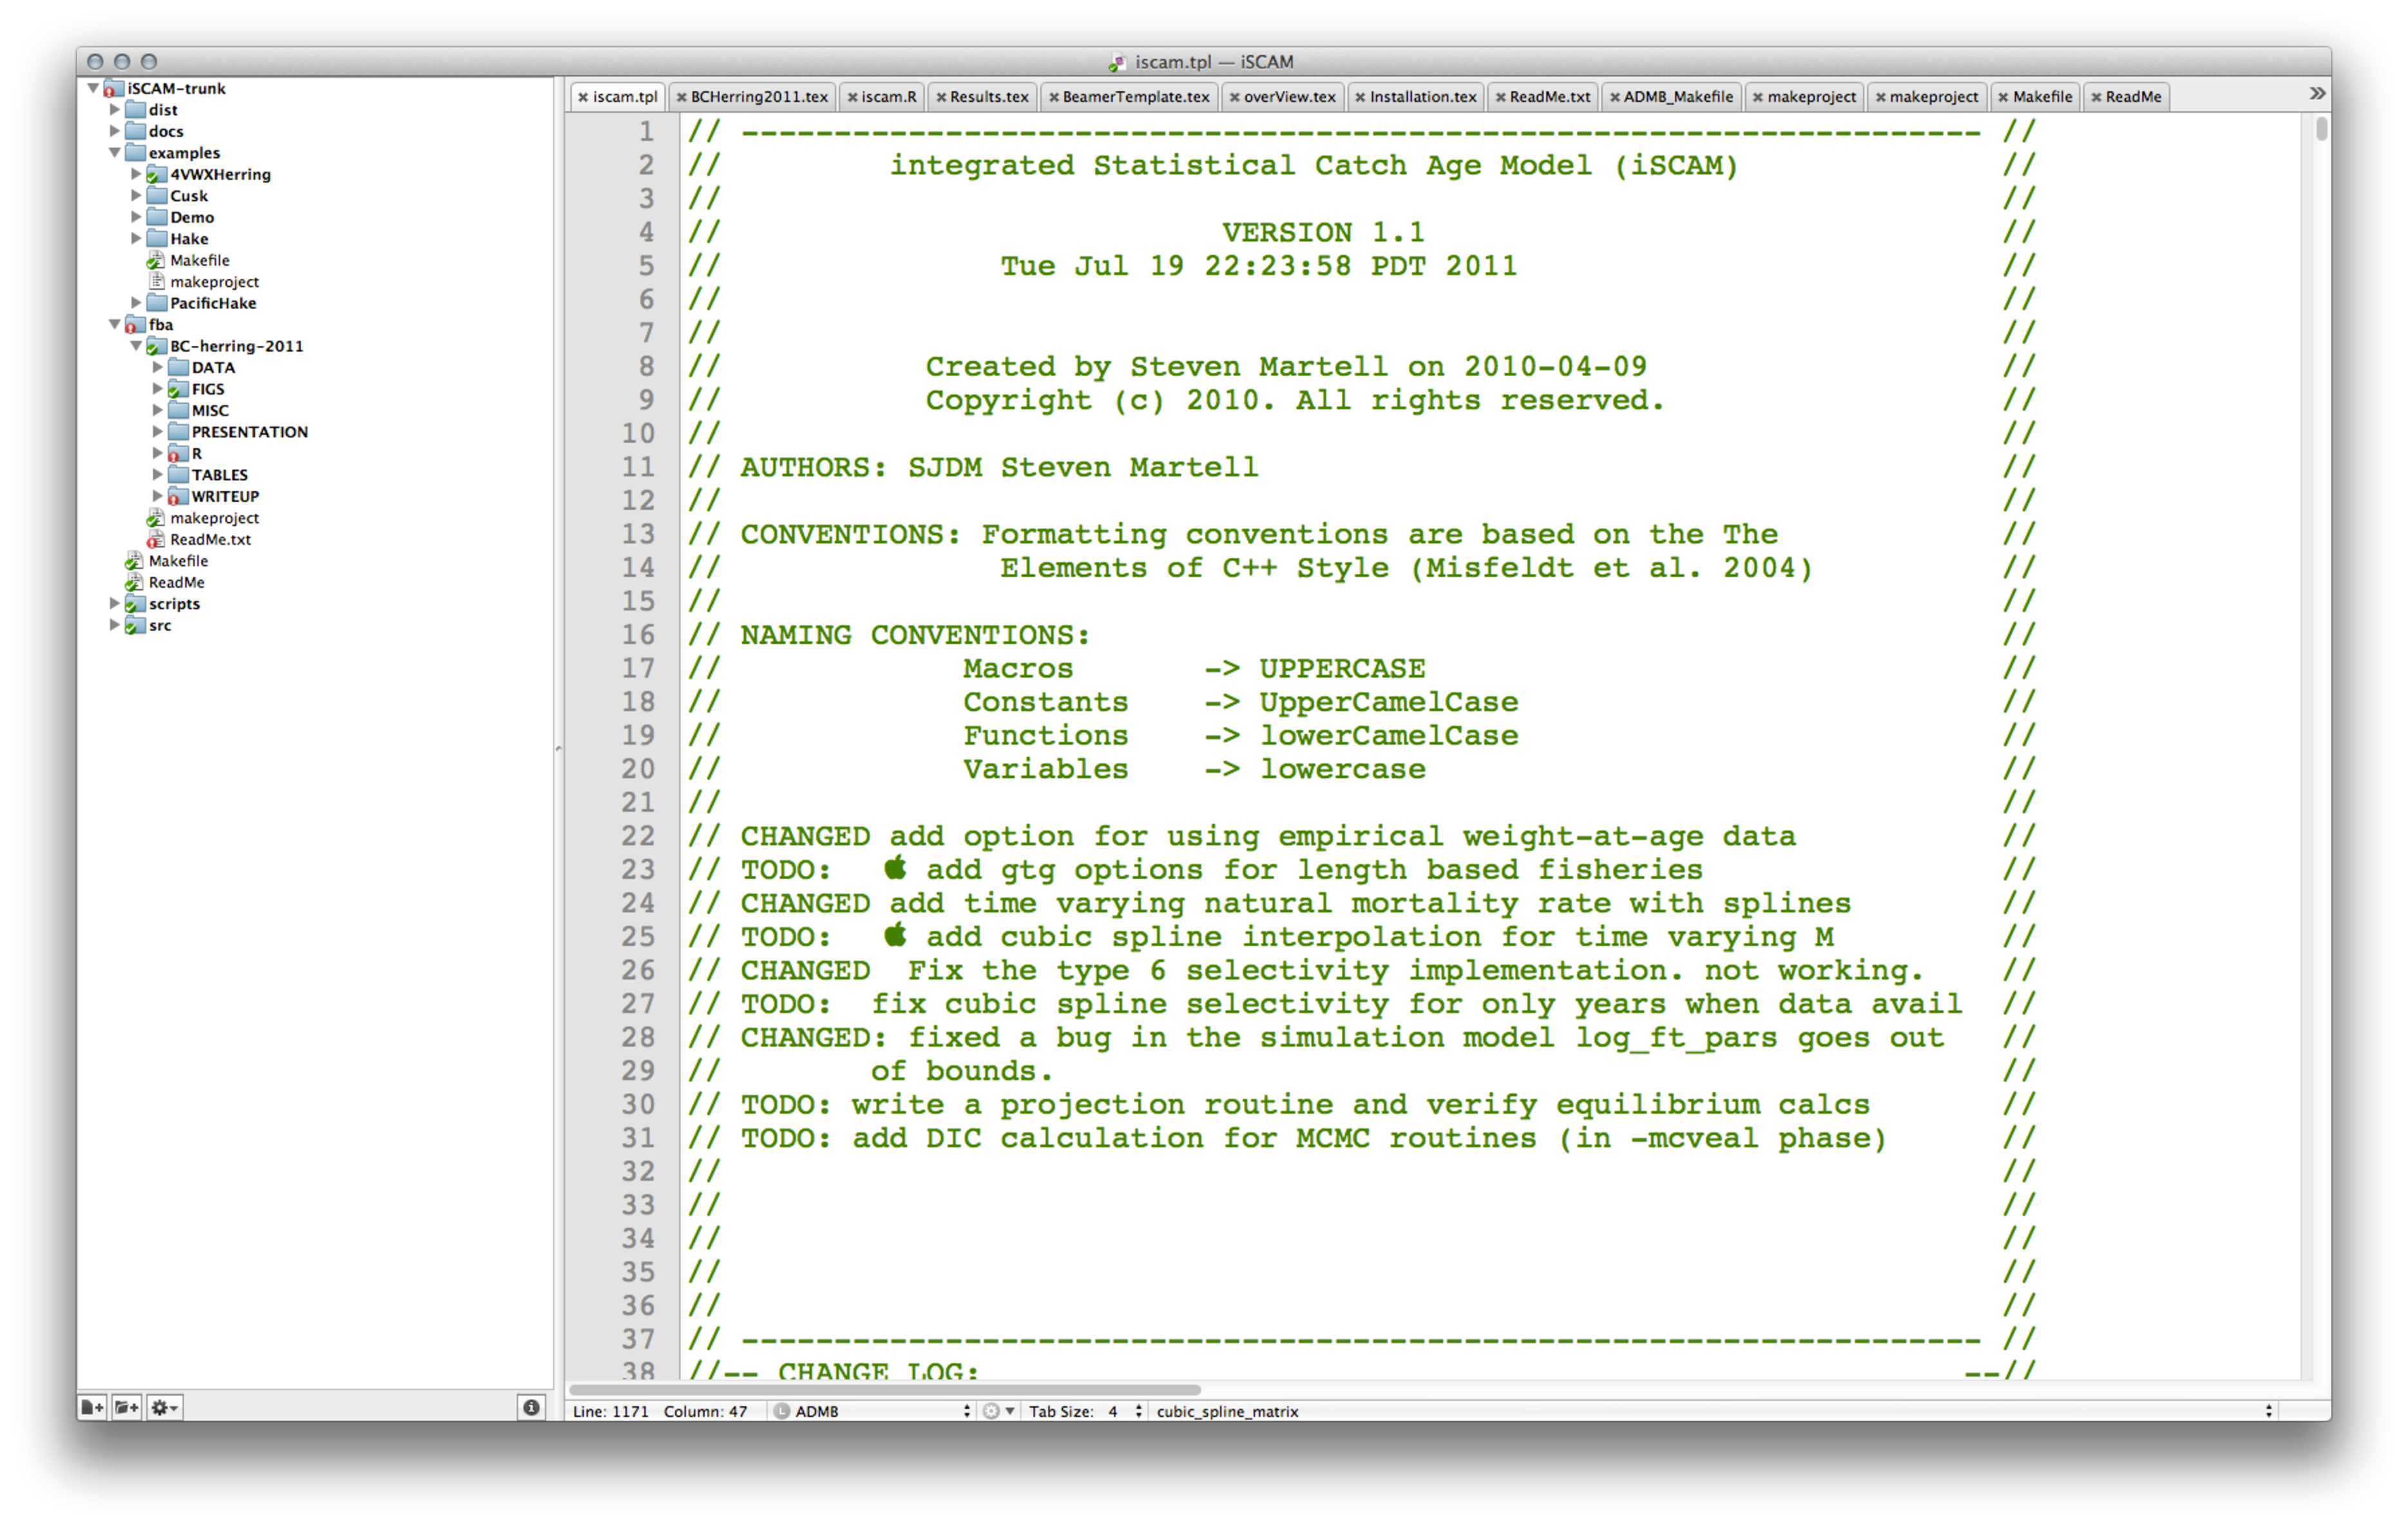
\includegraphics[height=2.5in]{screenCaptures/TextMate.pdf}
		\caption{Textmate on Mac OSX}
		\label{fig:screenCaptures_TextMate}
	\end{figure}
	}
\end{frame}
% subsection text_editors (end)

% section installation (end)
%!TEX root = /Users/stevenmartell/Documents/CURRENT PROJECTS/iSCAM-trunk/docs/iSCAM-guide/overView.tex

\section[Compiling]{Compiling Source Code} % (fold)
\label{sec:compiling_source_code}

\begin{frame}
	\frametitle{Compiling ADMB source code}
	What you need:
	\begin{itemize}
		\item C++ compiler (gcc recommended)
		\begin{itemize}
			\item Mac OSX: install Xcode from appstore
			\item Linux: \url{http://gcc.gnu.org/}
			\item Windoze: \url{http://www.mingw.org/}
		\end{itemize}
		\item ADMB libraries: \url{http://admb-project.org/downloads}
	\end{itemize}
	\vfill
	ADMB source code for \iscam\ found in:\\
	\texttt{./iSCAM-trunk/src/admb-code/}
\end{frame}

\begin{frame}
	\frametitle{Compiling from the command line}
	At the command line:
	\begin{itemize}[<+->]
		\item use cd to navigate to the ./iSCAM-trunk directory
		\item \underline{Linux or Mac OSX:} type Make
		\item \underline{Windows:} see \url{http://gnuwin32.sourceforge.net/packages/make.htm}
	\end{itemize}
	
	\only<1>{
	\vspace{-.25in}
	\begin{figure}[htbp]
		\centering
			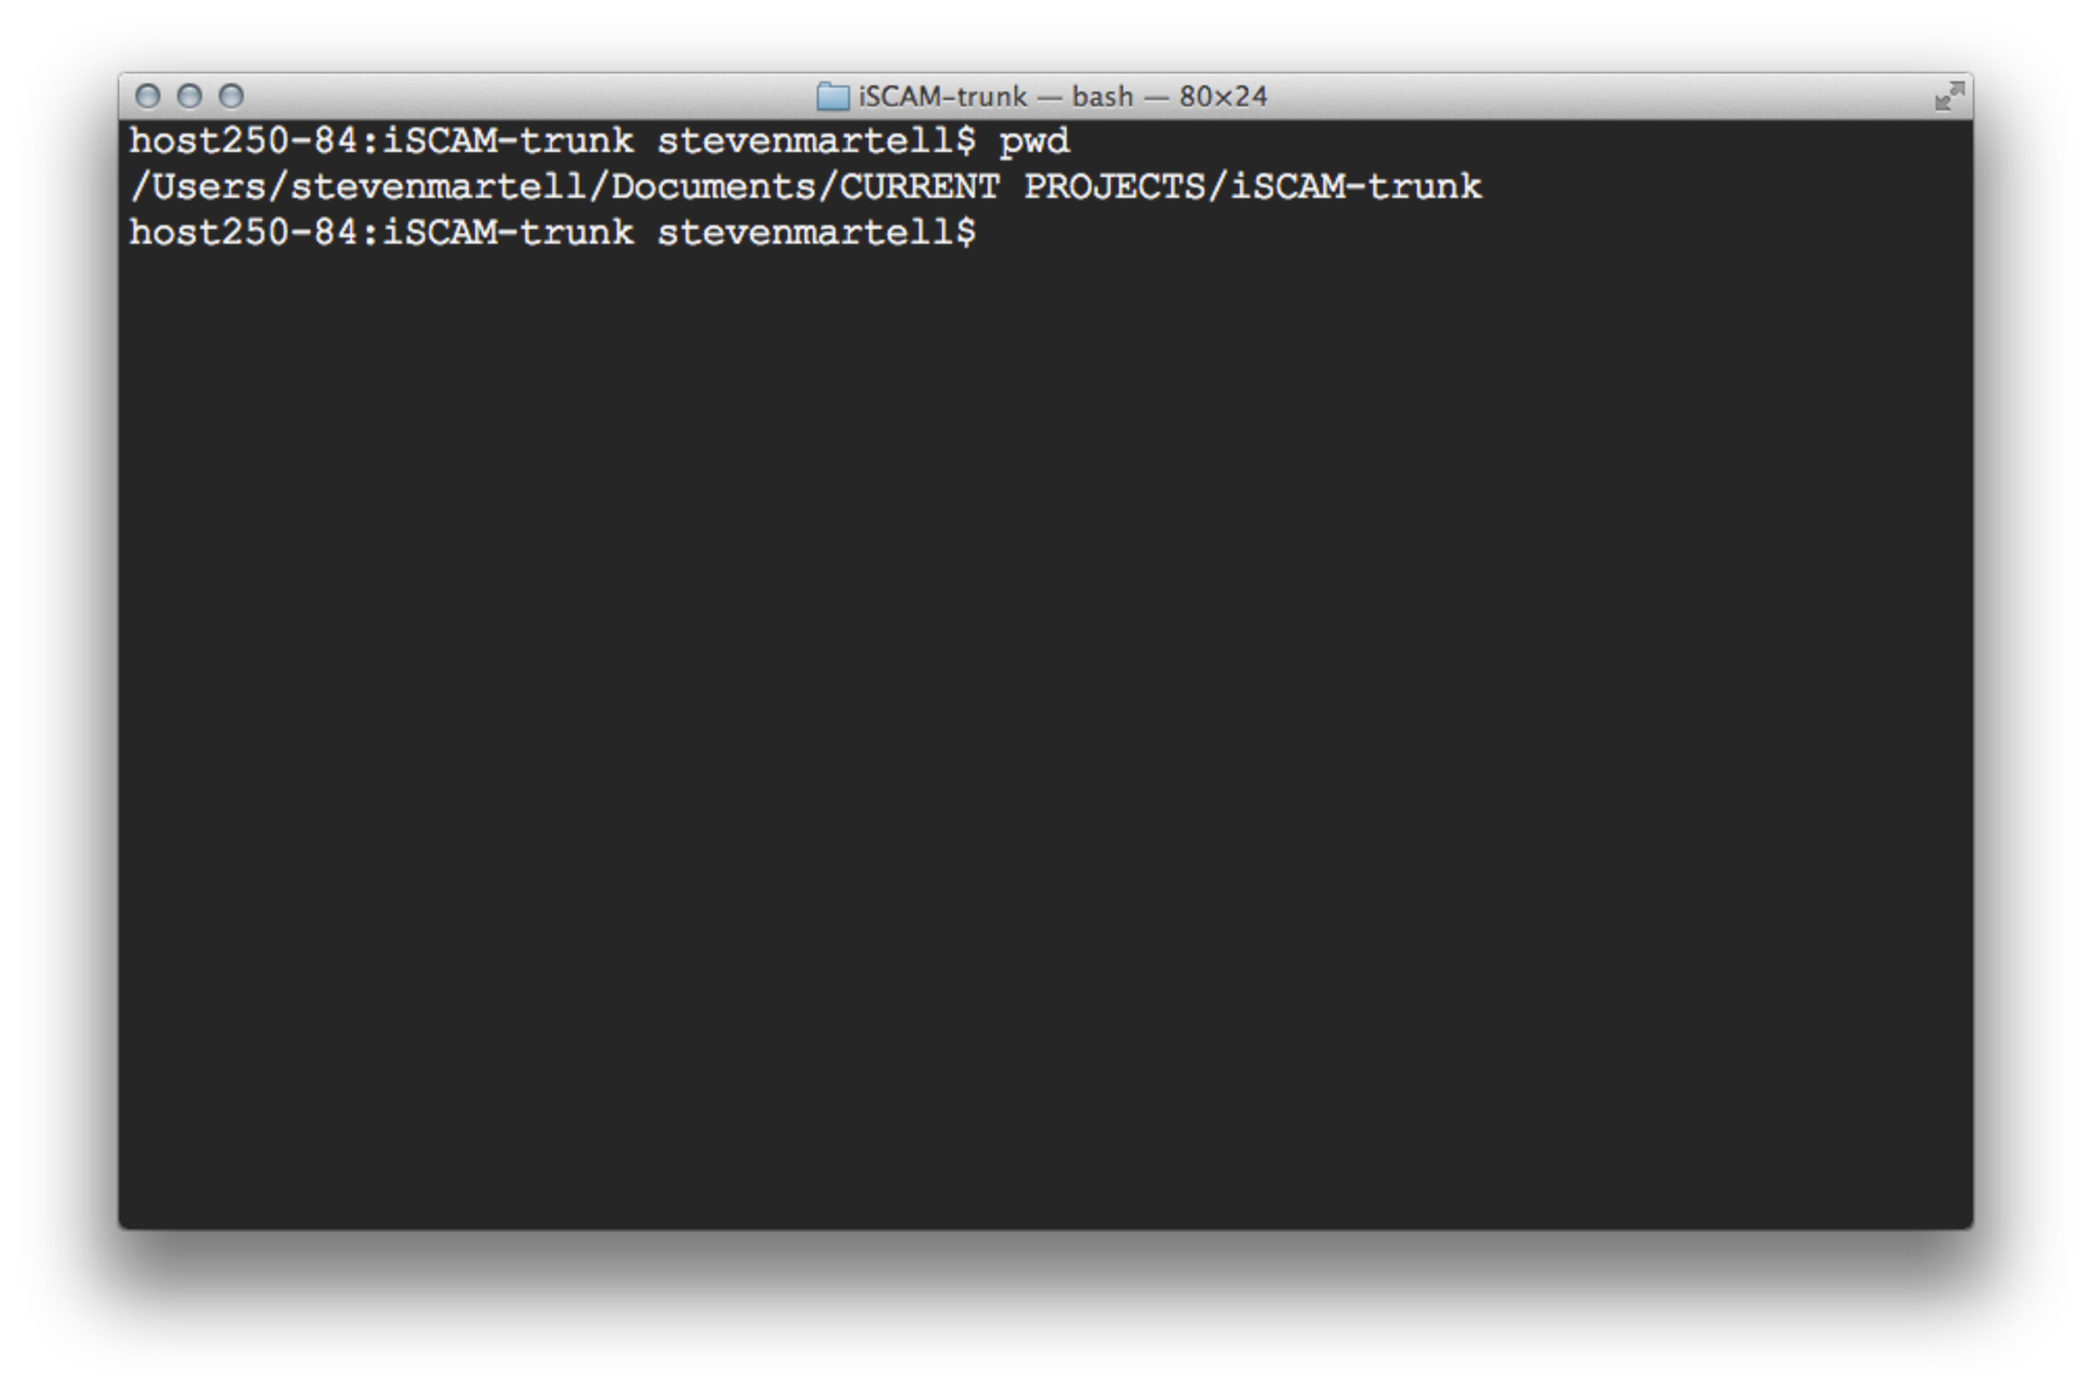
\includegraphics[height=2.5in]{screenCaptures/Term_iSCAM-trunk.pdf}
		\caption{}
		\label{fig:screenCaptures_Term_iSCAM-trunk}
	\end{figure}
	}
	\only<2>{
	\vspace{-.25in}
	\begin{figure}[htbp]
		\centering
			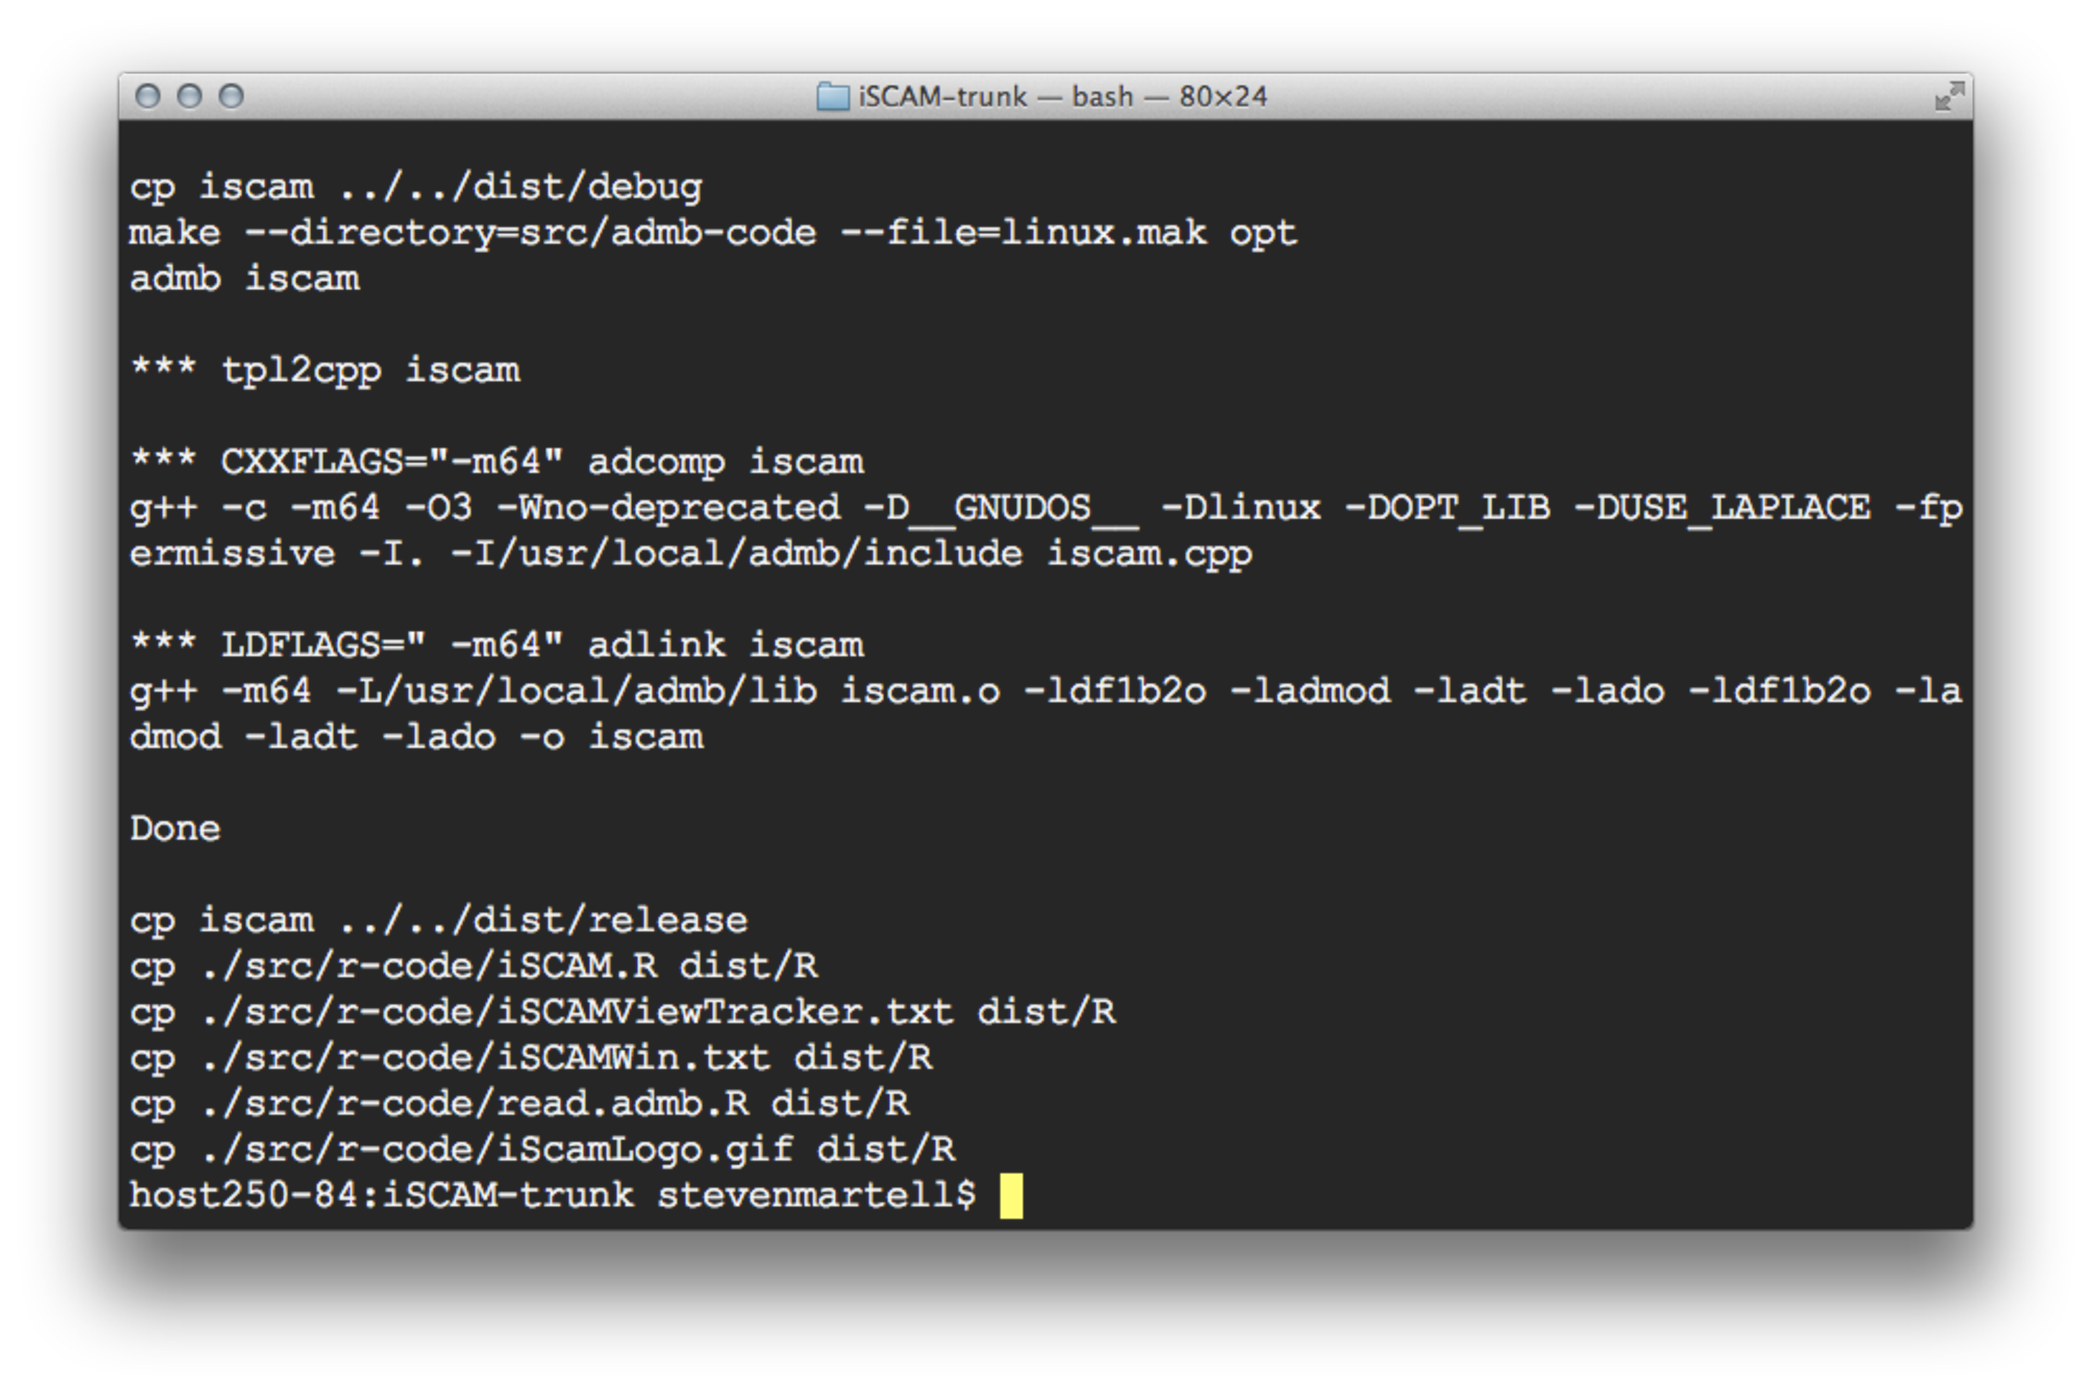
\includegraphics[height=2.5in]{screenCaptures/Term_make.pdf}
		\caption{}
		\label{fig:screenCaptures_Term_make}
	\end{figure}
	}
	\only<3>{
	\vspace{0.25in}
	Using the make file will compile the \iscam\ source code and place copies of the code in the distribution directory ("dist")
	}
\end{frame}

% section compiling_source_code (end)


%!TEX root = /Users/stevenmartell/Documents/CURRENT PROJECTS/iSCAM-trunk/docs/iSCAM-guide/overView.tex

\section{Running Examples} % (fold)
\label{sec:running_examples}
\begin{frame}
	\frametitle{Running examples}
	Examples in \texttt{iSCAM-trunk/examples}
	\begin{itemize}
		\item \texttt{Demo}
		\item \texttt{Hake}
	\end{itemize}
\end{frame}

\subsection{Demo Model} % (fold)
\label{sub:demo_model}


\begin{frame}
	\frametitle{Demo}
	\begin{itemize}
		\item The \texttt{Demo} directory is not present in the examples when you first checkout a copy of \iscam\ from the svn repository.
		\item To build the \texttt{Demo directory} cd to the examples directory and use \texttt{./makeproject Demo}
	\end{itemize}

\begin{figure}[htbp]
	\centering
		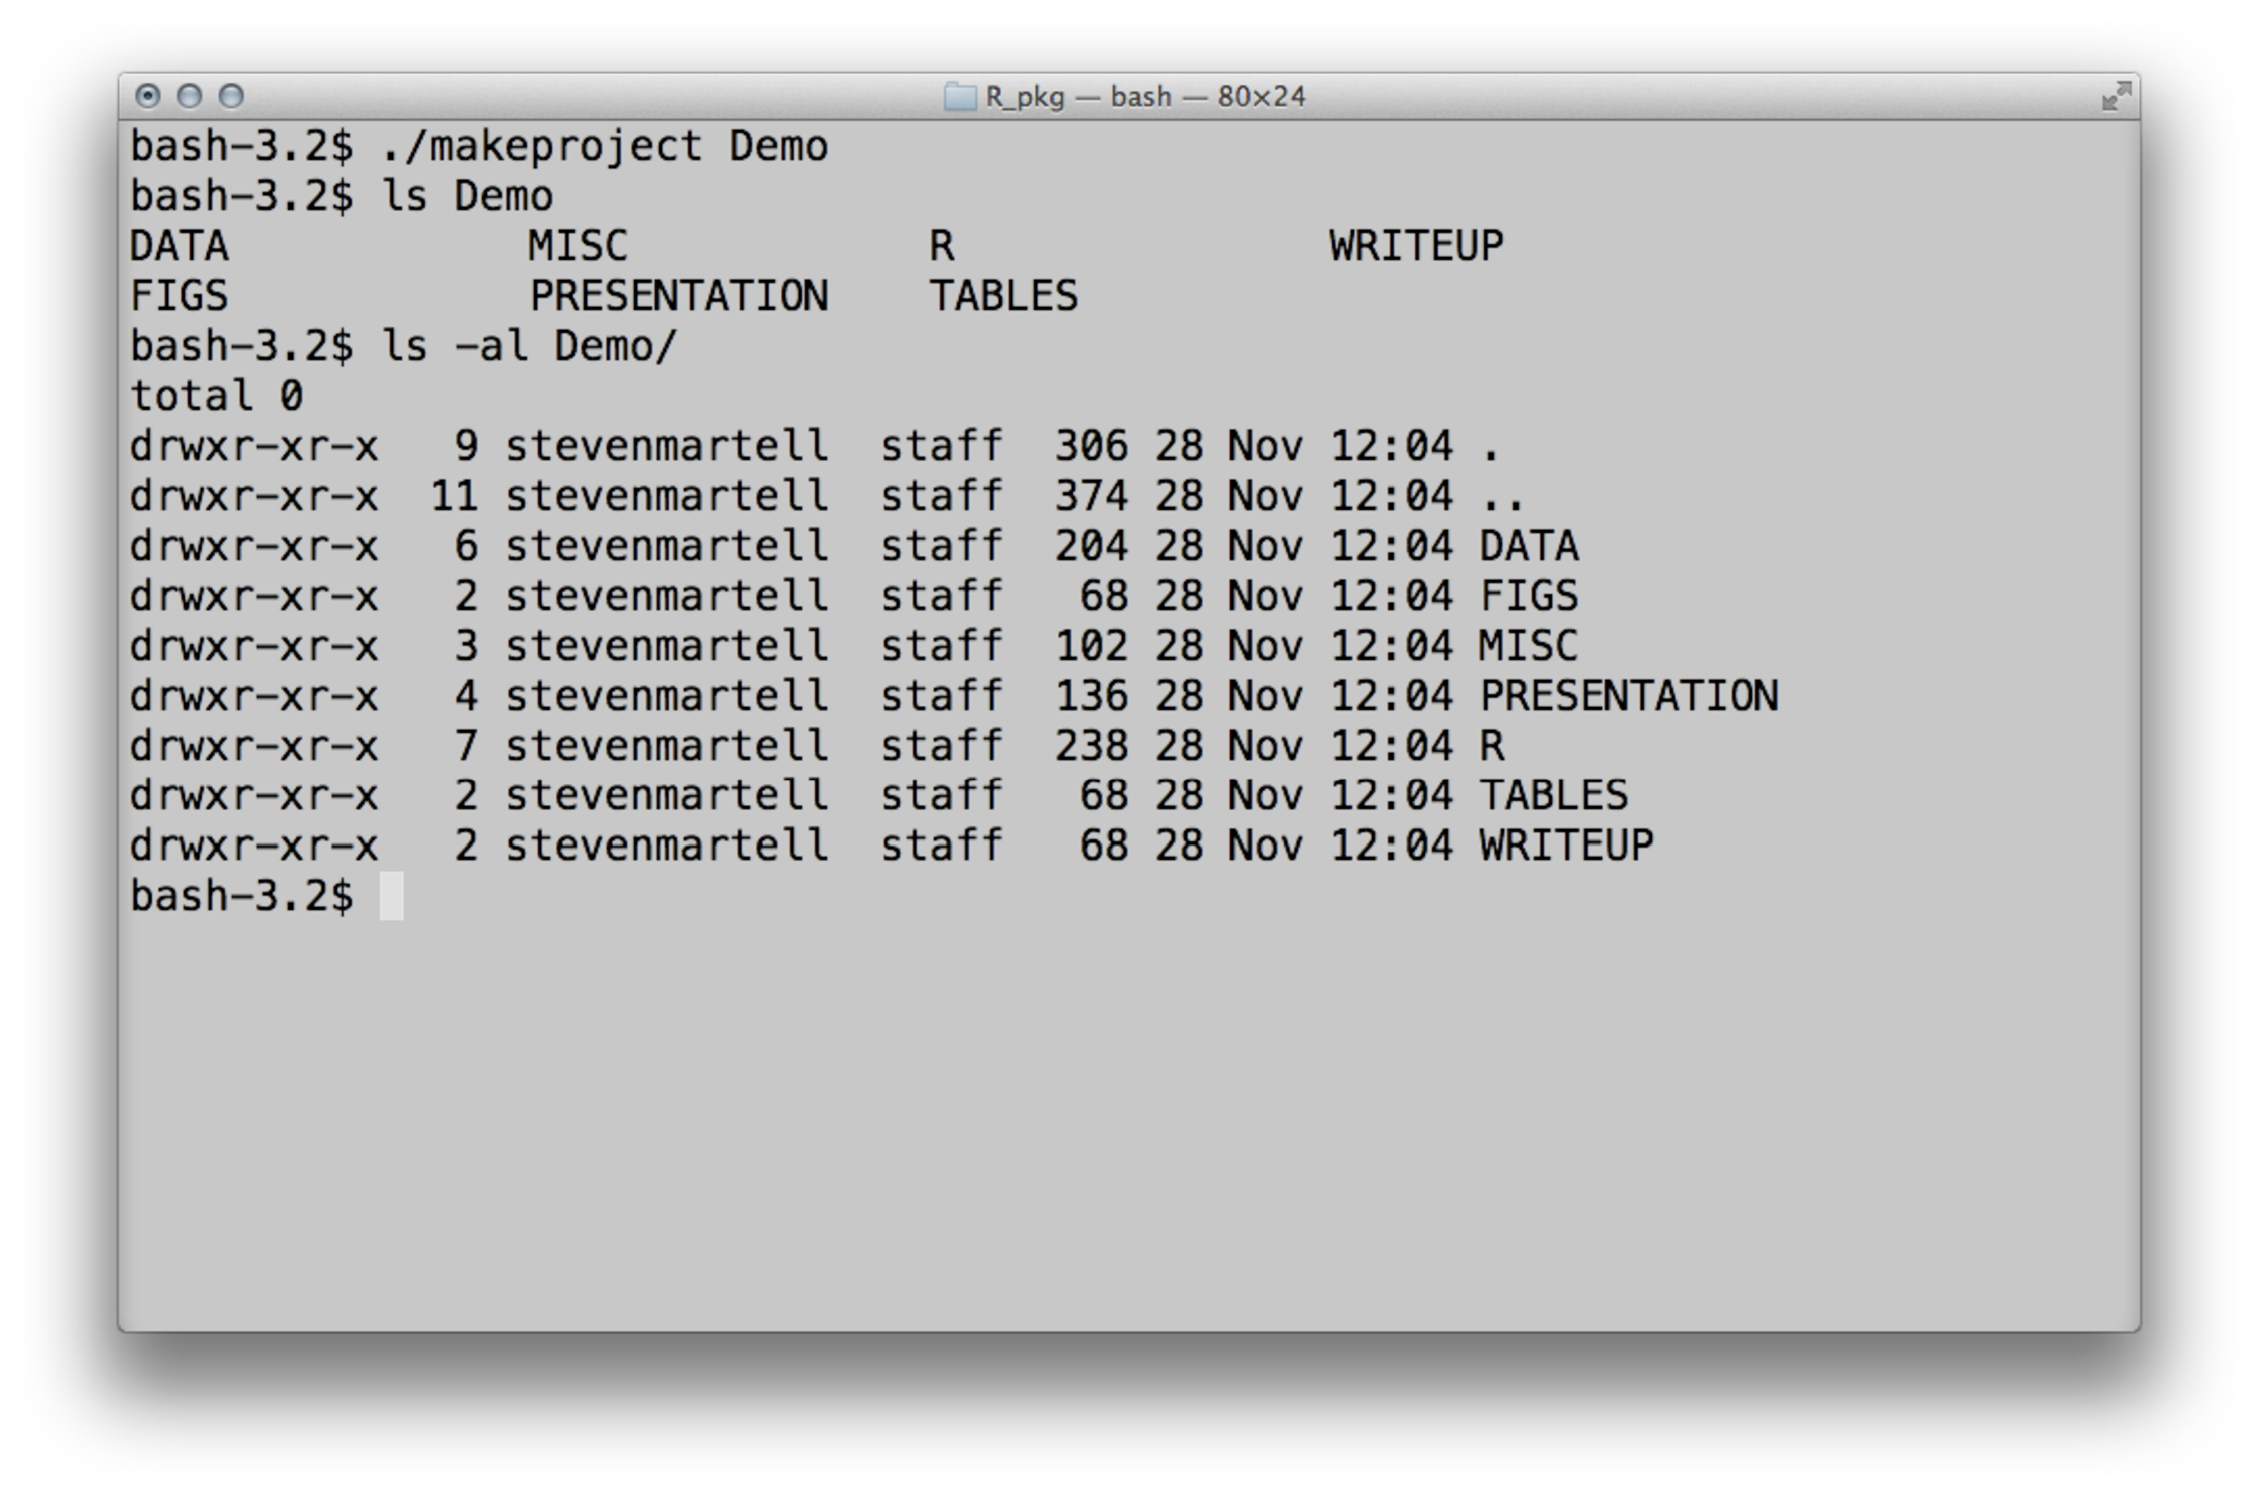
\includegraphics[height=1.75in]{screenCaptures/TermDemo.pdf}
	\caption{Using \texttt{makeproject} command to create \texttt{Demo}.}
	\label{fig:screenCaptures_TermDemo}
\end{figure}
\end{frame}

\begin{frame}
	\frametitle{Running the ADMB model in Demo}
	\begin{itemize}
		\item cd to the \texttt{examples/Demo/DATA} directory
		\item type \texttt{make} at the command line
	\end{itemize}
	\begin{figure}[htbp]
		\centering
			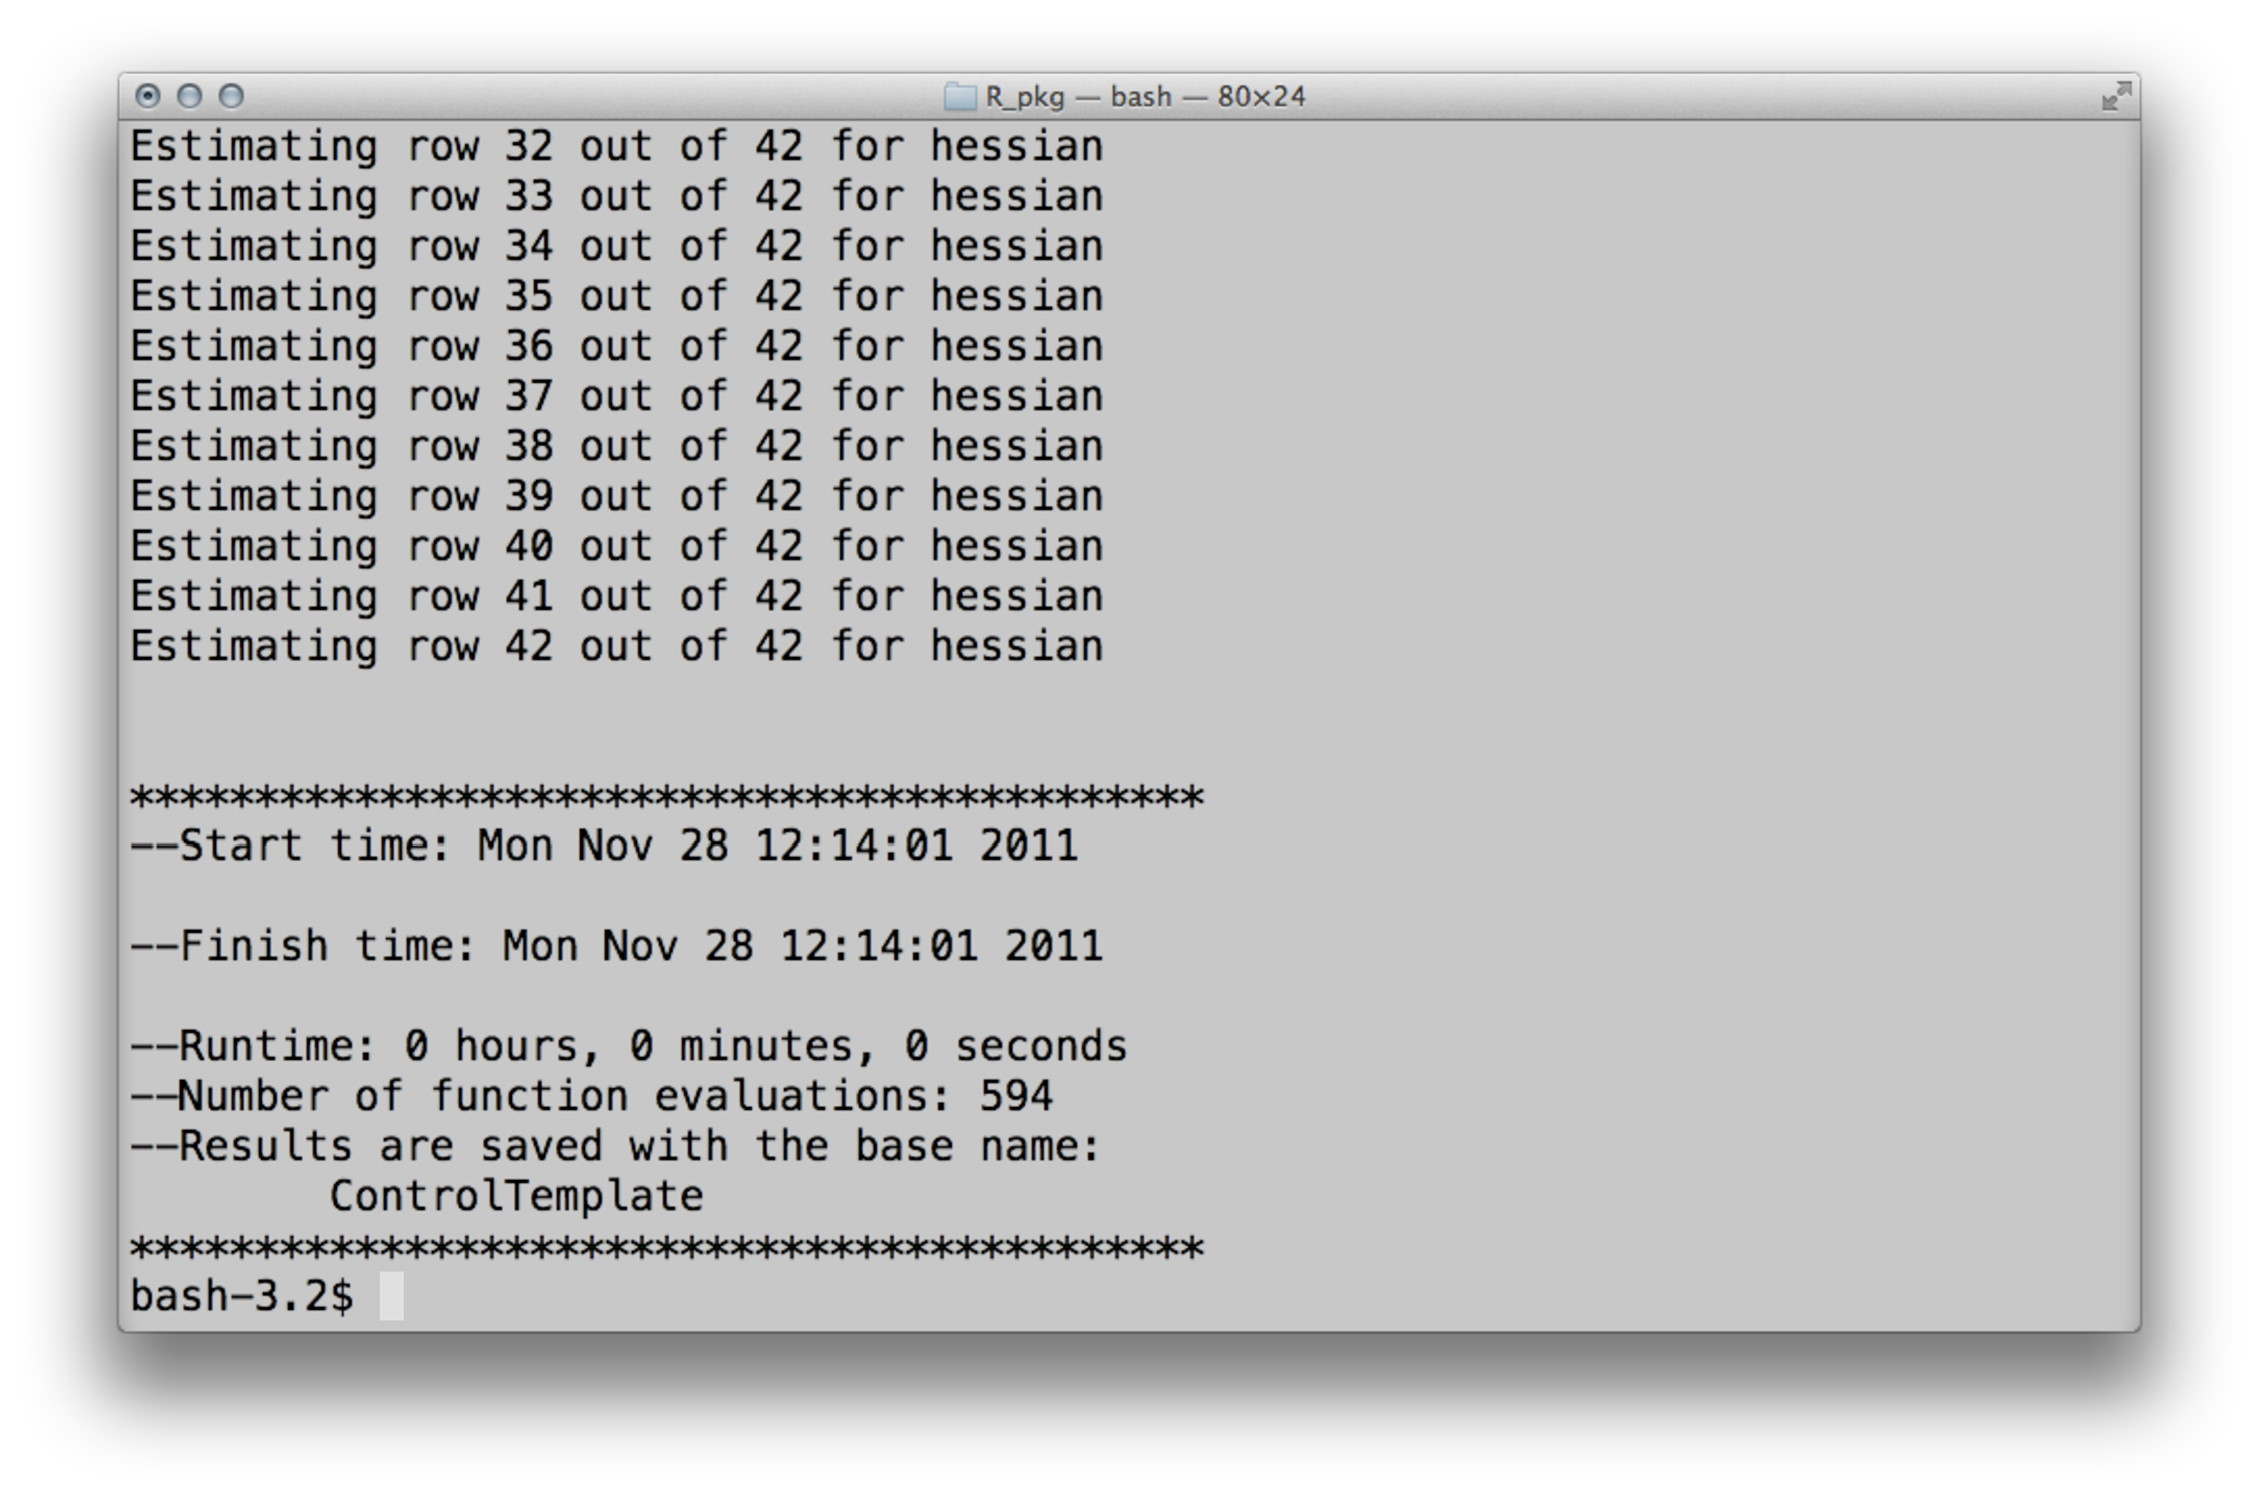
\includegraphics[height=1.75in]{screenCaptures/Term-catage.pdf}
		\caption{Terminal output after the Demo model has run}
		\label{fig:screenCaptures_Term-catage}
	\end{figure}
	
\end{frame}

% subsection demo_model (end)

\subsection{Makefile} % (fold)
\label{sub:makefile}
\begin{frame}[shrink=10]
	\frametitle{More on using \texttt{Makefile} }
	A makefile is a Unix utility that automatically executes a set of shell commands (rules). \underline{Target} rules are executed based on \underline{dependencies}.
	
	\begin{block}{Targets}
		\begin{itemize}
			\item all:  copy executable and run model with DAT \& ARG
			\item run:  copy executable and force a run
			\item mcmc: copy executable and run \texttt{mcmc} and \texttt{mceval}
			\item retro: copy executable and run retrospective R-script
			\item clean: remove executable \& other ADMB output files
		\end{itemize}
	\end{block}
	
	\begin{block}{Dependencies}
		\begin{itemize}
			\item EXEC - the name of the executable
			\item CTL - the name of the control file
		\end{itemize}
	\end{block}
	If the dependencies change then running make will execute the target scripts, otherwise there is no need to re-run the model.
\end{frame}

\lstset{language=make}
\begin{frame}[fragile]
	\frametitle{Setting up \texttt{Makefile}}
	User must supply variable Definitions in the Makefile:
	\begin{lstlisting}[cap=Makefile Defs]
	EXEC   = iscam
	prefix = ../../../dist
	DAT    = RUN.dat
	CTL    = ControlTemplate
	ARG    = 
	MCFLAG = -mcmc 10000 -mcsave 100 -nosdmcmc
	NR     = 4
	\end{lstlisting}
	\texttt{EXEC} is the program name, \texttt{prefix} is the (relative) path to the \texttt{dist} directory, \texttt{DAT} is the data file, \texttt{CTL} is the name of the control file, \texttt{ARG} optional command line argument (e.g., make run ARG="-nohess"), \texttt{MCFLAG} is the arguments for \texttt{make mcmc}, and \texttt{NR} is number of retrospective years (e.g., \texttt{make retro}). 
\end{frame}


\defverbatim[colored]\makesmart{%
\begin{lstlisting}[frame=single,emph={ga},emphstyle=\color{olive}]
bash-3.2$ make
make: Nothing to be done for `all'.
bash-3.2$  
\end{lstlisting}}%

\defverbatim[colored]\makearg{%
\begin{lstlisting}[frame=single,emph={ga},emphstyle=\color{olive}]
bash-3.2$ make run ARG = "-est -nox"
...
*******************************************
--Start time: Tue Nov 29 11:51:10 2011

--Finish time: Tue Nov 29 11:51:11 2011

--Runtime: 0 hours, 0 minutes, 1 seconds
--Number of function evaluations: 424
--Results are saved with the base name:
	ControlTemplate
*******************************************
bash-3.2$
\end{lstlisting}}%

\begin{frame}[fragile]
	\frametitle{Using \texttt{make} at the command line}
	\only<1>{
	Makefiles are smart, will only execute rules if the dependencies change:
	\vfill
	\makesmart
	}
	%%
	\only<2>{
	You can change the Makefile Defs at the command line:
	\vfill
	\makearg
	}
\end{frame}

\begin{frame}[fragile,shrink=30]
	\frametitle{Parallel execution with \texttt{Make}}
	Run multiple models in SUBDIR using: \texttt{make -j4}\\
	The "-j#" option specifies the number of processors to use.\\
	\texttt{SUBDIR} is the list of subdirectories in \texttt{DATA} (one for each model)\\
	\begin{lstlisting}[frame=single]
	## Makefile for running models
	## Author: steven martell <martell.steve@gmail.com>

	## Macros
	SUBDIR = CC PRD QCI SOG WCVI AREA27 AREA2W
	TARGET = 
	.PHONY: default $(SUBDIR) mcmc
	
	## Targets
	default: $(SUBDIR)
	$(SUBDIR):
		cd $@ && $(MAKE) $(TARGET)

	.PHONY: clean
	clean_files := $(foreach dir,$(SUBDIR),$(dir)/clean)

	clean: $(clean_files)
	$(clean_files):
		cd $(@D) && $(MAKE) clean
	\end{lstlisting}
	Sorry does not work on WINDOZE!
\end{frame}


% subsection makefile (end)

\begin{frame}
	\frametitle{Using \texttt{guiView}}
	In the R directory, source the iSCAM.R file in R $>$guiView()
	\begin{figure}[htbp]
		\centering
			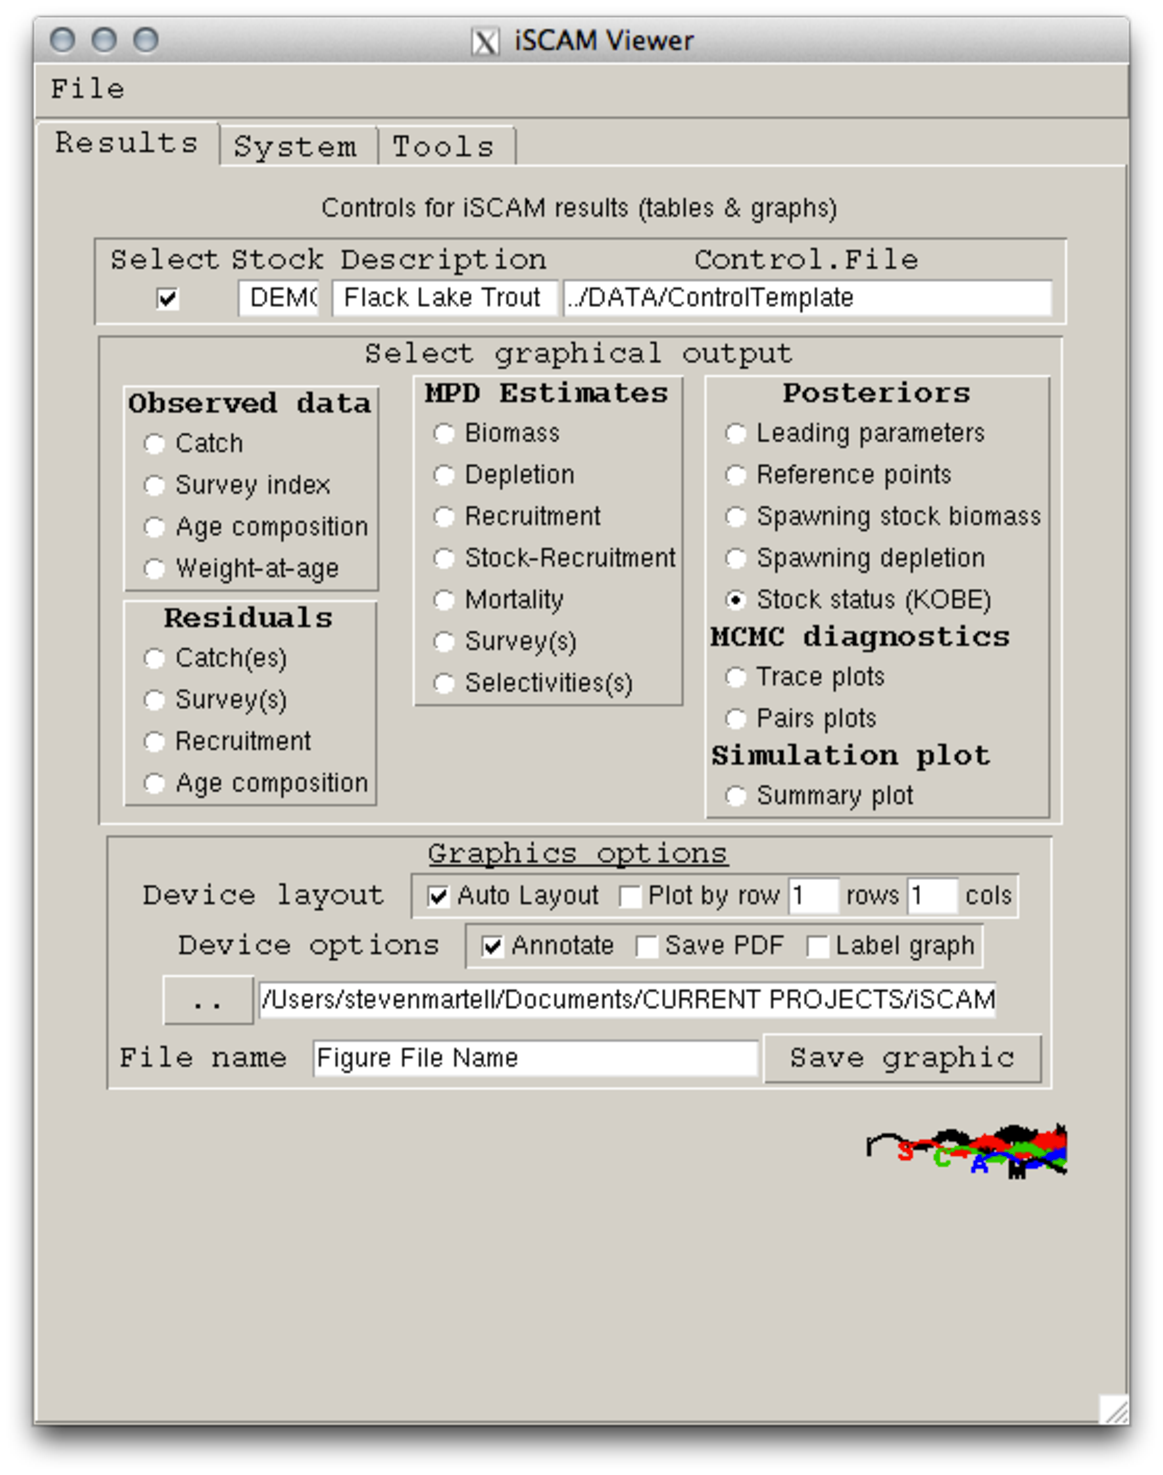
\includegraphics[height=2.5in]{screenCaptures/guiView.pdf}
		\caption{R gui for \iscam}
		\label{fig:screenCaptures_guiView}
	\end{figure}
	
\end{frame}


% section running_examples (end)
% 
% 
% 
% \begin{frame}
% \frametitle{Motivation}
% \begin{block}
% {Why Beamer?}
% Does anybody need an introduction to Beamer? I don't think so.
% \end{block}
% \end{frame}
% %
% \begin{frame}
% \frametitle{Example of a Theorem}
% \begin{theorem}
% The quick brown fox jumps over the lazy dog.
% \end{theorem}
% \end{frame}
% %
% \begin{frame}[fragile] % Notice the [fragile] option %
% \frametitle{Verbatim}
% \begin{example}[Putting Verbatim]
% \begin{verbatim}
% \begin{frame}
% \frametitle{Outline}
% \begin{block}
% {Why Beamer?}
% Does anybody need an introduction to Beamer?
% I don't think so.
% \end{block}
% % Extra carriage return causes problem with verbatim %
% \end{frame}\end{verbatim} 
% \end{example}
% \end{frame}
%  
% \begin{frame}[fragile]  % notice the fragile option, since the body
% 			% contains a verbatim command
% Example of the \verb|\cite| command to give a reference is below:
% Example of citation using \cite{key1} follows on.
% \end{frame}
%  
% \begin{frame}
% \frametitle{References}
% \footnotesize{
% \begin{thebibliography}{99}
%  \bibitem[Label1, 2010]{key1} Author's name (1987)
%  \newblock Title of the paper.
%  \newblock \emph{Journal Name} 55(4), 765 -- 799.
% \end{thebibliography}
% }
% \end{frame}
%  
% \begin{frame}
% \centerline{The End}
% \end{frame}
% End of slides
\end{document}

